\chapter{Ambition, Fuel to Success}

This chapter follows Jim Rohn's lecture, as preserved in the curated LazyingArt LLC playlist, closely in narrative order. No usable board images survive for this talk, so the equations and diagrams below are cautious transcript-backed reconstructions of the lecture's inner mechanics rather than transcriptions of visible blackboard work. The underlying structure is nevertheless remarkably crisp: wish becomes desire, desire acquires discipline, dreams develop pull, success is decomposed into inner and outer terms, service becomes investment, and small actions propagate through the whole network of life.

\section{From Wish to Disciplined Eager Desire}

The lecture opens with a puzzle. Ambition is said to be a mystery, and then immediately reduced to a dictionary phrase: an eager desire for distinction, power, or fame. But the lecturer is not satisfied with the dictionary. He asks what the word ``eager'' actually does for us. We are eager for birthdays, games, performances, old friends, shopping, excitement. Yet we rarely say that we are eager for a better life, a better family, or more money. ``And that's a problem,'' because in the lecture's logic a better life requires precisely that kind of eagerness.

The first distinction, then, is between a wish and a desire. A wish names an outcome from a distance. A desire begins to rearrange conduct. The lecture's weight-loss and money examples are important because they are concrete. We all know what it is to wish vaguely; the point is that change does not begin there.

\begin{definition}
In the logic of this lecture, ambition is disciplined, eager desire: a desire strong enough to bind tomorrow's hope to today's conduct.
\end{definition}

The first law of the chapter is therefore
\begin{equation}
\text{ambition}=\text{disciplined, eager desire}.
\end{equation}
The next law distinguishes passive wanting from operative wanting:
\begin{equation}
\text{wish} \not\Rightarrow \text{change},
\qquad
\text{desire}+\text{discipline}\Rightarrow \text{change}.
\end{equation}
If we want the meeting tomorrow, we prepare today. If we want college money later, we save today. If we want a better life tomorrow, we begin to work on it today:
\begin{equation}
\text{better life tomorrow} \Rightarrow \text{work today}.
\end{equation}

A compact summary of the opening progression is
\begin{equation}
W \longrightarrow D \xrightarrow{\text{discipline}} A,
\end{equation}
where \(W\) is wish, \(D\) is desire, and \(A\) is ambition.

The lecture's opening mechanism is simple enough to diagram, and the point of the diagram is not decoration but order. The speaker is teaching us how one state becomes another.

\begin{figure}
\centering
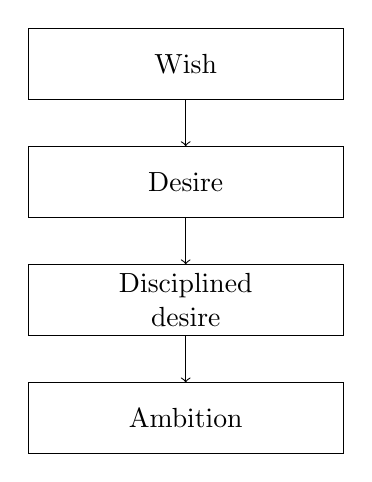
\begin{tikzpicture}[x=1cm,y=1cm]
\draw (0,0) rectangle (4,0.9);
\node at (2,0.45) {Wish};
\draw[->] (2,0) -- (2,-0.6);
\draw (0,-1.5) rectangle (4,-0.6);
\node at (2,-1.05) {Desire};
\draw[->] (2,-1.5) -- (2,-2.1);
\draw (0,-3.0) rectangle (4,-2.1);
\node[align=center] at (2,-2.55) {Disciplined\\ desire};
\draw[->] (2,-3.0) -- (2,-3.6);
\draw (0,-4.5) rectangle (4,-3.6);
\node at (2,-4.05) {Ambition};
\end{tikzpicture}
\end{figure}

Only after this opening conversion does the lecturer make the temporal claim explicit:
\begin{equation}
\text{ambition}=\text{minute-by-minute, day-by-day mentality}.
\end{equation}
Ambition is not a mood that visits us once. It is a repeated alignment of present action with future aim.

\subsection{Question \& Answer}

\paragraph{Question.} What turns a wish into ambition?

\paragraph{Answer.} Not intensity by itself. The lecture's answer is that ambition appears when desire acquires backbone. A wish says, ``I would like the result.'' Ambition says, ``Because I want the result, I will alter what I do now.'' The crucial operator is discipline.

\section{Dreams, Pull Power, and the Finished Future}

Once ambition has been defined inwardly, the lecture widens the frame. Why does one small group seem to build and enjoy fortune while a much larger group struggles merely to earn a living? The striking thing is that the lecturer does not answer first with economics or circumstance. He answers with dreams. Among the many conditions that shape a life, the ability to dream is singled out as having the greatest potential power for good.

Dreams are not treated as misty wishes. They are projections of the kind of life we want to lead, and as such they exert force. The lecture's next relations may be written as
\begin{equation}
\text{well-defined dream}\Rightarrow \text{pull power},
\qquad
\text{fuzzy future}\Rightarrow \text{little pull power}.
\end{equation}
Schematically,
\begin{equation}
\text{dream vividness}\uparrow \Rightarrow \text{motivational pull}\uparrow.
\end{equation}
This is what the lecture means when it says that dreams can drive us and make us skip over obstacles. The obstacle is not denied. Its effective importance is altered by the pull of a clear future.

The historical examples matter here. The pioneers crossing mountains, the immigrants arriving with defined goals, the image of California seen while still climbing the peak: all of this is a way of turning a moral exhortation into mechanics. To survive the pass, one must already be living toward the far side. The future must be seen as finished in advance. In the lecturer's language, one hears the cheers before the race is over.

The governing idea is
\begin{equation}
\text{dreams} \Rightarrow \text{creative force stronger than obstacles}.
\end{equation}
The phrase is strong, but its meaning is precise. Obstacles still exist; what changes is the balance of forces in the mind of the actor.

\subsection{Question \& Answer}

\paragraph{Question.} Why do well-defined dreams pull harder than obstacles push?

\paragraph{Answer.} Because definition gives the future usable shape. A vague hope cannot order sacrifice. A vivid future can. Once the end is seen in advance, the hardship is no longer an isolated burden; it becomes a stage of a route.

\section{Franklin's Three Principles of Success}

The lecture now pivots from pioneers and immigrants to Ben Franklin. This is a shift from grand image to practical doctrine. Franklin appears not chiefly as inventor or statesman, but as one of the first American writers of self-making. The transition is important. Ambition must now be translated from inspiration into repeatable law.

The first principle is that happiness does not come in large blocks of finished success, but in small advantages hammered out day by day. Let \(a_n\) denote the \(n\)-th small advantage, and let \(B_N\) denote the built achievement after \(N\) such gains. Then the lecture's structure can be represented by
\begin{align}
B_N &= \sum_{n=1}^{N} a_n,\\
a_n &= \text{a small advantage won on day }n.
\end{align}
This is not meant as literal arithmetic. It is a faithful mathematical rendering of the lecture's compounding idea. Big achievement is built out of repeated local gains.

The second principle is Franklin's phrase that life is plastic. In the lecture, this means
\begin{equation}
\text{life is plastic}\Rightarrow \text{self and environment are moldable}.
\end{equation}
The dream provides a form in advance, and then one works the material of life every minute, every day, every month, every year. The lecture therefore connects Franklin back to the earlier dream imagery: first the form is seen, then the material is shaped.

The third principle is stated in a deliberately surprising way:
\begin{equation}
\text{success}=\text{pleasure}.
\end{equation}
This does not mean pleasure as distraction. It means that if the present activity is empty, then the final trophy cannot fully redeem it. The lecturer reinforces this with a very practical notebook criterion: at the end of the day, what have we done that made the day good? If we can write such things down consistently, a pattern of success begins to appear before any public triumph is complete.

Franklin's three principles may therefore be restated as
\begin{align}
\text{big achievement} &= \sum \text{small advantages},\\
\text{life is plastic} &\Rightarrow \text{it can be shaped},\\
\text{success} &= \text{pleasure along the way}.
\end{align}
This is one of the lecture's most important transitions. Ambition is no longer only a matter of heat. It is now given daily form.

\section{William James, the Inner Ideal, and the Word ``Until''}

From Franklin the lecture moves to William James, and with James the tone becomes more explicitly philosophical. Pragmatism is introduced not as an abstract school but as a habit of asking what an idea does, what use it has, what practical result it yields. Then comes the chapter's cleanest decomposition of success:
\begin{align}
S &= I + O,\\
I &= \text{inner ideal followed persistently with courage},\\
O &= \text{outer achievement related to that ideal}.
\end{align}
The lecture immediately qualifies the sum by ranking the terms:
\begin{equation}
I \succ O.
\end{equation}
The first term is more important than the second. The inner ideal is the governing condition because once that inner aim is abandoned, outer achievement ceases to have the same meaning.

Schematically, the lecture's logic may be written as
\begin{align}
I=0 &\Rightarrow S \text{ collapses in the strong sense},\\
I>0,\ O=0 &\Rightarrow S \text{ remains possible and already begins},\\
I>0,\ O>0 &\Rightarrow S \text{ is success in both inward and outward form}.
\end{align}
This is not a visible board equation, but it is a cautious standard reconstruction of the lecturer's exact point: success is already active in a life that has not abandoned its governing ideal.

The next move is crucial. The lecture leans heavily on a single word: ``until.'' Read until the skill changes. Go to the seminars until the thing makes sense. Practice until it is right. Stay with the process until one learns, changes, and grows. Thus
\begin{equation}
\text{do it until} \Rightarrow \text{learn, change, grow}.
\end{equation}
And in the lecture's cumulative phrasing,
\begin{equation}
\text{step by step}+\text{piece by piece}+\text{book by book}+\text{seminar by seminar}
\Rightarrow
\text{progress}.
\end{equation}
The force of ``until'' is that it turns duration into an operator. Time is no longer a reason to quit; it is the medium in which the ideal is proved.

\subsection{Question \& Answer}

\paragraph{Question.} How can one already count as successful before the outer achievement is complete?

\paragraph{Answer.} Because the lecture refuses to identify success with the last visible prize alone. If the inner ideal remains active and is being pursued with courage, then success has already begun to exist in the present. The outward completion matters, but it does not create the inward term from nothing.

\section{Small Changes, Daily Evidence, and the Social Field of Success}

Having defined success in Jamesian terms, the lecture asks the natural next question: what outward evidence appears while the work is still underway? The answer is strikingly modest. We first see change in little things, not major things. It appears in sleep, mood, greeting, schedule, household presence, and the tone of ordinary encounter.

The central rule is
\begin{equation}
\text{change within} \Rightarrow \text{change around}.
\end{equation}
A companion rule sharpens it:
\begin{equation}
\text{respond differently to life} \Rightarrow \text{life responds differently to you}.
\end{equation}
This is still the same chapter-long structure. A local shift changes the field in which later events occur.

\paragraph{Worked example.} The lecture's example of going to bed earlier can be written as a simple update chain:
\begin{align}
d_1 &= \text{go to bed a little earlier},\\
d_2 &= \text{rise in a better mood},\\
d_3 &= \text{begin the day more effectively},\\
d_4 &= \text{work with other people more gracefully}.
\end{align}
Thus
\begin{equation}
d_1 \Rightarrow d_2 \Rightarrow d_3 \Rightarrow d_4.
\end{equation}
The point is not the specific habit. The point is propagation. One local correction alters the next local state.

The lecture then broadens the field still further. Smile at the person in traffic. Offer the cheerful greeting at the office. Embrace the family before collapsing on the sofa. These are not throwaway bits of moral uplift. They are the visible outward evidence of inward reform.

From here the lecturer makes a claim that is nearly axiomatic:
\begin{equation}
\text{each of us needs all of us}.
\end{equation}
This is his denial that success can be solitary. Even the person who appears to work alone is supported by the patience, tolerance, and service of others. Gratitude is therefore not merely a nicety. It is a truthful description of how work is actually carried.

The lecture then inserts a long but important motivational beat: stories of people who have already traveled the road. The orphanage-to-millionaire story, Jesse Jackson's message of ``I am somebody,'' the insistence that lasting motivation is backed by education, and the travel analogy in which we seek advice from someone who has already been where we intend to go, all serve one function. They convert admiration into method. The lesson is that stories are usable because they carry routes, not just excitement.

A transcript-backed compression of this beat is
\begin{equation}
\text{right knowledge} \Rightarrow \text{self-motivation}.
\end{equation}
And the lecture's striking final phrase for this transition is that the journey of pursuit itself can become the best alarm clock in the world. By the time Joseph Epstein is introduced, the ground has been prepared: ambition is no longer merely desire; it is educated desire that has learned how to renew itself.

\section{Ambition, Not Greed: Constructive and Destructive Desire}

Joseph Epstein supplies the next bridge:
\begin{equation}
\text{ambition}=\text{fuel of achievement}.
\end{equation}
But the lecturer immediately qualifies the term. Ambition is not greed. It is not avarice. It is not success at another person's expense:
\begin{equation}
\text{ambition}\neq \text{greed},
\qquad
\text{ambition}\neq \text{avarice}.
\end{equation}

The distinction is then sharpened with admirable economy:
\begin{equation}
\text{desire}=\text{what you want},
\qquad
\text{ambition}=\text{how you get there}.
\end{equation}
Desire is compatible with either good or bad method. It may want the tallest building in town. But there are then two possible paths. One path destroys the neighboring buildings. The other designs, plans, gathers a team, endures the weather, and builds upward.

\begin{equation}
\text{destructive desire}\Rightarrow \text{tear others down},
\qquad
\text{constructive ambition}\Rightarrow \text{build upward}.
\end{equation}

\begin{figure}
\centering
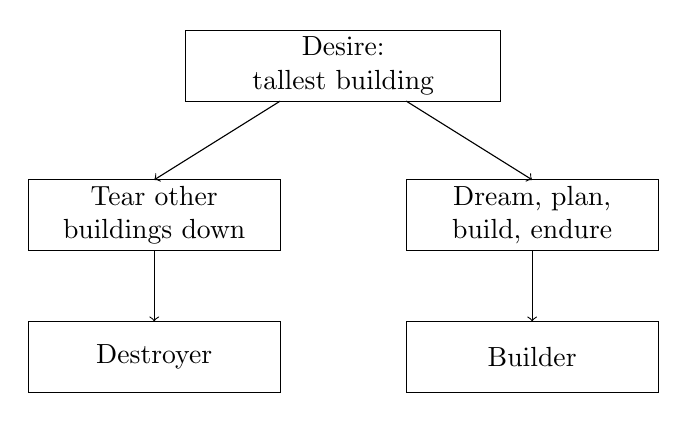
\begin{tikzpicture}[x=1cm,y=1cm]
\draw (2,0) rectangle (6,0.9);
\node[align=center] at (4,0.45) {Desire:\\ tallest building};
\draw[->] (3.2,0) -- (1.6,-1.0);
\draw[->] (4.8,0) -- (6.4,-1.0);

\draw (0,-1.9) rectangle (3.2,-1.0);
\node[align=center] at (1.6,-1.45) {Tear other\\ buildings down};

\draw (4.8,-1.9) rectangle (8.0,-1.0);
\node[align=center] at (6.4,-1.45) {Dream, plan,\\ build, endure};

\draw[->] (1.6,-1.9) -- (1.6,-2.8);
\draw[->] (6.4,-1.9) -- (6.4,-2.8);

\draw (0,-3.7) rectangle (3.2,-2.8);
\node[align=center] at (1.6,-3.25) {Destroyer};

\draw (4.8,-3.7) rectangle (8.0,-2.8);
\node[align=center] at (6.4,-3.25) {Builder};
\end{tikzpicture}
\end{figure}

This is why the Judas example is introduced. Judas ends with money, but not with ambition, because the process itself is corrupting. The lecture is not judging only the final possession. It is judging the geometry of the pursuit and the person produced by it.

\subsection{Question \& Answer}

\paragraph{Question.} How is ambition different from greed if both seem to want more?

\paragraph{Answer.} Greed wants gain without regard for the damage done to others or to the self. Ambition, as the lecture defines it, accepts the discipline of construction. It builds, plans, serves, and endures. The difference lies not only in the object sought, but in the path taken.

\section{Enlightened Self-Interest, Service, and the Law of Deserving}

The lecture's last long movement gathers everything into a more operational system. Self-interest, we are told, is not itself a flaw. The flaw begins when self-interest is left unenlightened. In the lecture's compact form,
\begin{equation}
\text{enlightened self-interest}\Rightarrow \text{benefit by service to others},
\end{equation}
whereas
\begin{equation}
\text{self-interest at the expense of others}\Rightarrow \text{greed / evil}.
\end{equation}
Hence the strong contrast:
\begin{equation}
\text{enlightened self-interest}\Rightarrow \text{wealth},
\qquad
\text{self-preservation alone}\Rightarrow \text{poverty}.
\end{equation}

The story of the broke man in a hotel room, still spending hours each night helping feed the homeless, matters here. It is not sentiment but evidence. Service alters the social field, and the altered field later returns work, opportunity, and support. The lecture is thinking causally.

From here it passes to giving:
\begin{equation}
\text{if you wish to receive, you must give}.
\end{equation}
The next step is decisive:
\begin{equation}
\text{giving}=\text{investment},
\qquad
\text{investment}\Rightarrow \text{return multiplied}.
\end{equation}
This is the logic behind ``do more than you get paid for.'' In the lecture, this is not merely moral counsel; it is an investment rule:
\begin{equation}
\text{do more than you get paid for} \Rightarrow \text{investment in future return}.
\end{equation}
And so too with sales:
\begin{equation}
\text{make a sale} \Rightarrow \text{make a living},
\qquad
\text{serve beyond the sale} \Rightarrow \text{make a fortune}.
\end{equation}

Then comes one of the lecture's cleanest laws:
\begin{equation}
\text{life responds to deserve, not need}.
\end{equation}
The rejected law is
\begin{equation}
\text{need} \not\Rightarrow \text{reap}.
\end{equation}
The accepted law is
\begin{equation}
\text{plant} \Rightarrow \text{reap}.
\end{equation}
The soil metaphor is exact. Need does not move the soil. Seed does. Therefore the lecture expands seed into practical inputs:
\begin{equation}
\text{seed}+\text{effort}+\text{discipline}+\text{service}\Rightarrow \text{return}.
\end{equation}
What appears as moral rhetoric is really a causal rule: bring the field something to work on.

The same pattern governs searching:
\begin{equation}
\text{search} \Rightarrow \text{find},
\qquad
\text{searching} \Rightarrow \{\text{ideas},\text{hope},\text{contacts},\text{inspiration}\}.
\end{equation}
If we want to find, we must enter the places in which finding becomes possible: the seminar, the library, the bookstore, the class, the training.

Now the lecture makes its final systems-claim:
\begin{equation}
\text{one discipline affects another},
\qquad
\text{all disciplines affect each other}.
\end{equation}
In its broadest form,
\begin{equation}
\text{everything affects everything else}.
\end{equation}
This gives both the negative and positive cascades:
\begin{align}
\text{every letdown} &\Rightarrow \text{affects the rest},\\
\text{every new discipline} &\Rightarrow \text{affects the rest}.
\end{align}

\begin{figure}
\centering
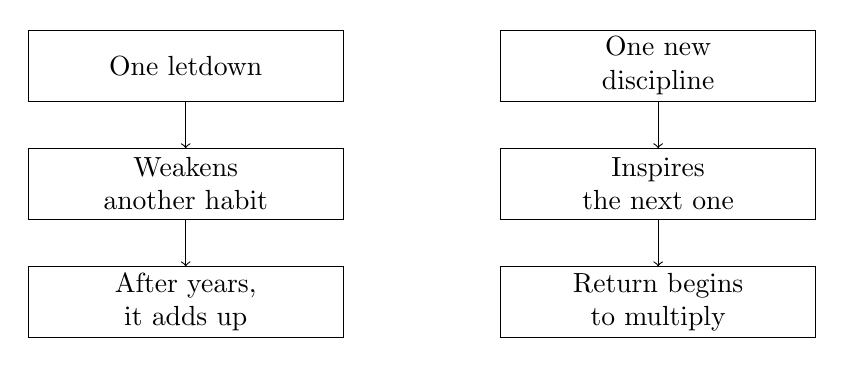
\begin{tikzpicture}[x=1cm,y=1cm]
\draw (0,0) rectangle (4,0.9);
\node[align=center] at (2,0.45) {One letdown};
\draw[->] (2,0) -- (2,-0.6);
\draw (0,-1.5) rectangle (4,-0.6);
\node[align=center] at (2,-1.05) {Weakens\\ another habit};
\draw[->] (2,-1.5) -- (2,-2.1);
\draw (0,-3.0) rectangle (4,-2.1);
\node[align=center] at (2,-2.55) {After years,\\ it adds up};

\draw (6,0) rectangle (10,0.9);
\node[align=center] at (8,0.45) {One new\\ discipline};
\draw[->] (8,0) -- (8,-0.6);
\draw (6,-1.5) rectangle (10,-0.6);
\node[align=center] at (8,-1.05) {Inspires\\ the next one};
\draw[->] (8,-1.5) -- (8,-2.1);
\draw (6,-3.0) rectangle (10,-2.1);
\node[align=center] at (8,-2.55) {Return begins\\ to multiply};
\end{tikzpicture}
\end{figure}

\paragraph{Worked example.} The lecture gives a concrete positive chain:
\begin{align}
c_1 &= \text{walk around the block},\\
c_2 &= \text{eat right},\\
c_3 &= \text{buy a book},\\
c_4 &= \text{keep a journal},\\
c_5 &= \text{develop skills}.
\end{align}
Hence
\begin{equation}
c_1 \Rightarrow c_2 \Rightarrow c_3 \Rightarrow c_4 \Rightarrow c_5.
\end{equation}
This is why the lecture insists on the least action:
\begin{equation}
\text{smallest action} \Rightarrow \text{momentum},
\end{equation}
and then immediately adds the next law:
\begin{equation}
\text{accomplishment} \Rightarrow \text{inspiration for the next accomplishment}.
\end{equation}

The lecture ends not with abstraction alone but with autobiography. The surroundings, the world, the general conditions may remain the same, but the person changes. Books are read, classes are taken, philosophy is refined, and the outcome shifts. In the lecture's closing form:
\begin{equation}
\text{same surroundings}+\text{changed philosophy}\Rightarrow \text{different life}.
\end{equation}

\subsection{Question \& Answer}

\paragraph{Question.} Why does life respond to deserve rather than need?

\paragraph{Answer.} Because the lecture treats life as a field rather than as a pitying judge. A field does not answer complaint; it answers seed. Need names absence. Deserving names what has actually been planted into the world: effort, service, willingness, and disciplined action.

\subsection{Question \& Answer}

\paragraph{Question.} How can the least action matter if the problems are large?

\paragraph{Answer.} Because disciplines are coupled. A single act is not isolated; it changes mood, schedule, confidence, competence, and the probability of the next act. The smallest action matters precisely because it is not the last act. It is the first term in a cascade.

\section{Summary}

We can now see the full architecture of the lecture. Ambition begins as disciplined, eager desire and immediately acquires a temporal form: today must be altered for tomorrow to change. Dreams then supply pull, especially when the future is well defined and vividly seen in advance. Franklin translates ambition into small daily advantages, moldability, and pleasure in the process. James decomposes success into an inner ideal and an outer achievement, while insisting on the primacy of the first term and on the discipline of ``until.'' The lecture then returns to ordinary evidence: small changes in habit, better relations with other people, gratitude for the support field, and the education of motivation by stories and examples. Finally, ambition is rescued from greed, self-interest is enlightened by service, deserving replaces mere need, and discipline is revealed as a coupled network in which the smallest new action can alter the rest. In this sense the lecture's deepest mathematical image is one of compounding structure. A life changes because one disciplined act becomes the condition of the next.